\documentclass{article}
\usepackage{graphicx} % Required for inserting images
\usepackage{amsmath}
\usepackage{hyperref}
\usepackage{amsthm}
\usepackage{amssymb}
\title{Executive summary: Plug-in estimation of Schrodinger bridges
}
\author{Viresh Pati}
\date{January 2025}

\begin{document}

\maketitle

\section{Paper Details}
Aram-Alexandre Pooladian and Jonathan Niles-Weed. "Plug-in estimation of Schrödinger bridges" \textit{arXiv.}2024. \href{https://arxiv.org/abs/2408.11686}{[arxiv]}

\section{Repository}
The authors provide code at \href{https://github.com/APooladian/SinkhornBridges}{[this github]} which runs on some benchmarks. We should be able to adapt for NSF challenge.
\newpage
\section{High-level problem}
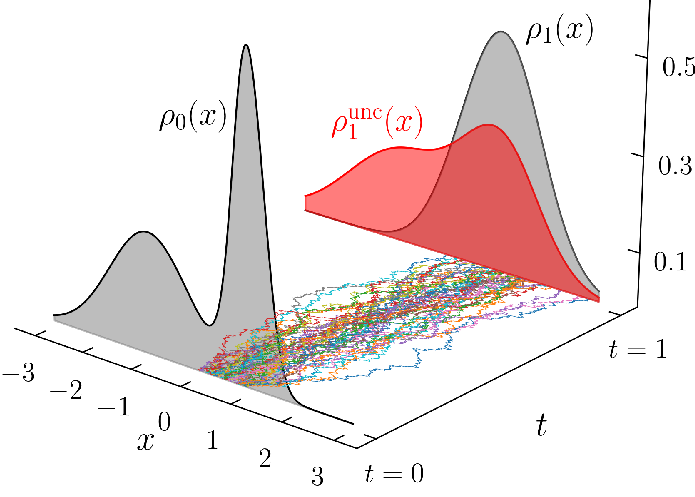
\includegraphics[width=\textwidth, height=0.4\textheight]{Smooth Schrodinger Bridges/1-Figure1-1.png}
When we have two probability distributions $\mu$ and $\nu$ , the Schrodinger Bridge gives a most likely stochastic process from source distribution $\mu$ to  target distribution $\nu$. That is,
\begin{itemize}
    \item We want to transform samples from $\mu$ into samples from $\nu$ by simulating a diffusion over time.
    \item The Schrodinger Bridge is the process that minimizes relative entropy.

\end{itemize}
Existing methods to estimate that time-dependent diffusion require heavy iterative SDE simulation or neural networks. The authors propose a simple plug-in estimator:
\begin{itemize}
    \item Solve the static entropic optimal transport between $\mu$ and $\nu$ once.
    \item Use these entropic OT potentials to directly plug in a drift formula that defines the Schrodinger bridge over time.

\end{itemize}
\section{Intuition behind the technique}
\begin{itemize}
    \item Entropic OT (via Sinkhorn's Algortim) is already a soft coupling between $\mu$ and $\nu$. 
    \item Schrodinger bridge is also an entropic construction in that it is the minimal-entropy stochastic process that connects $\mu$ and $\nu$.
    \item This work shows that the "entropic penalty" that arises in the classical entropic OT problem is the same in the Schrodinger bridge problem, so the dual potentials from Sinkhorn effectively store all the needed information to diffuse between distributions.
\end{itemize}
\section{Results}
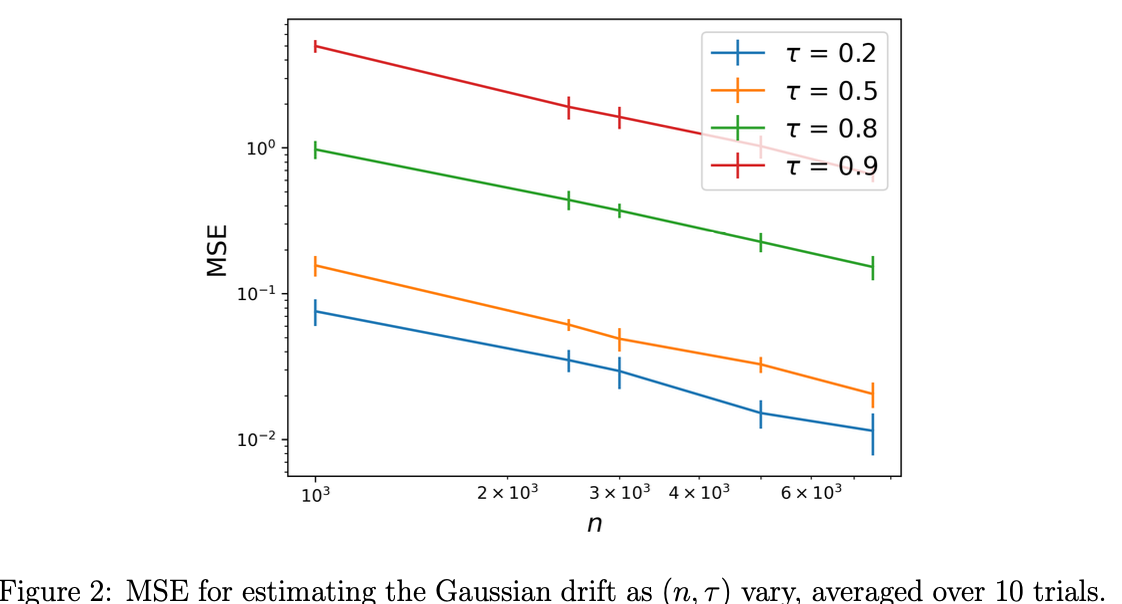
\includegraphics[width=\textwidth, height=0.4\textheight]{Smooth Schrodinger Bridges/Drift.png}
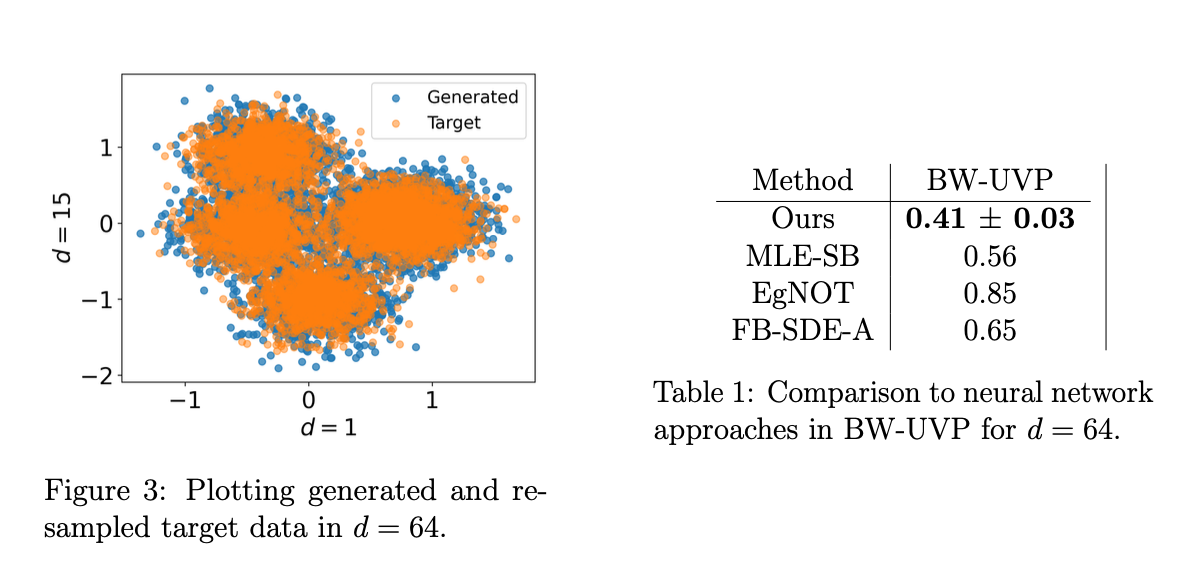
\includegraphics[width=\textwidth, height=0.4\textheight]{Smooth Schrodinger Bridges/SynthData.png}
\section{Some more background and detail}
\subsection{Optimal Transport}
In classical optimal transport, we seek a joint distribution $\pi$ with marginals $\mu$ and $\nu$ that minimizes the average cost $|x-y|^2$ of pairing $x\in \mu$ and $y\in \nu$. \\
Entropic OT adds a small entropic penalty that makes $\pi$ spread out and keeps the problem strictly convex, solvable by Sinkhorn's algorithm.

$$\int |x-y|^2 \pi (dx, dy) + \epsilon \mathrm{KL}(\pi || \mu  \otimes v)$$
\[\text{Note:$\pi(x,y)$ is a coupling, we'll say "how much mass from $x\in \mu$ is shipped to point $y\in \nu$ "}\]

Instead of directly finding joint $\pi$ we can use a dual-formulation to find two scalar function $f$ that lives on the support of $\mu$ and $g$ that lives on the support of $\nu$ . We will omit detail for brevity, but Sinkhorn's algorithm updates $f$ and $g$ based on each other until convergence, and you end with approximations for each sample in the distributions.\\
\subsection{From potentials to Schrodinger Bridge }
It turns out the potentials from entropic OT encode the correction terms needed to steer a Brownian motion from $\mu$ to $\nu$. That is, reading off potentials from the Sinkhorn solution and plugging into a known formula for drift (deterministic part) of an SDE between $\mu$ and $\nu $ is precisely the Schrodinger Bridge.
\section{Application to vessel trajectories}

We can treat each data snapshot as a discrete empirical distribution, run EOT and plug dual potentials to get a drift that flows one vessel shape into the other in time. We may want to parameterize multiple time-steps in a neural network, and/or do a latent encoding of raw vessel data to obtain $\mu$ and $\nu$.\\

\textit{On runtime:} naive Sinkhorn is $O(kn^2)$ where $k $ is the number of iterations to convergence (there are some small optimizations possible and the paper also divides out some constraint tolerances so this is a loose bound). And then there is usually negligible $O(nt)$ drift where $t$ is the discrete number of steps. Sinkhorn's is also highly parallelizable.
 
\end{document}
